% Options for packages loaded elsewhere
\PassOptionsToPackage{unicode}{hyperref}
\PassOptionsToPackage{hyphens}{url}
%
\documentclass[
]{article}
\usepackage{amsmath,amssymb}
\usepackage{lmodern}
\usepackage{iftex}
\ifPDFTeX
  \usepackage[T1]{fontenc}
  \usepackage[utf8]{inputenc}
  \usepackage{textcomp} % provide euro and other symbols
\else % if luatex or xetex
  \usepackage{unicode-math}
  \defaultfontfeatures{Scale=MatchLowercase}
  \defaultfontfeatures[\rmfamily]{Ligatures=TeX,Scale=1}
\fi
% Use upquote if available, for straight quotes in verbatim environments
\IfFileExists{upquote.sty}{\usepackage{upquote}}{}
\IfFileExists{microtype.sty}{% use microtype if available
  \usepackage[]{microtype}
  \UseMicrotypeSet[protrusion]{basicmath} % disable protrusion for tt fonts
}{}
\makeatletter
\@ifundefined{KOMAClassName}{% if non-KOMA class
  \IfFileExists{parskip.sty}{%
    \usepackage{parskip}
  }{% else
    \setlength{\parindent}{0pt}
    \setlength{\parskip}{6pt plus 2pt minus 1pt}}
}{% if KOMA class
  \KOMAoptions{parskip=half}}
\makeatother
\usepackage{xcolor}
\usepackage{color}
\usepackage{fancyvrb}
\newcommand{\VerbBar}{|}
\newcommand{\VERB}{\Verb[commandchars=\\\{\}]}
\DefineVerbatimEnvironment{Highlighting}{Verbatim}{commandchars=\\\{\}}
% Add ',fontsize=\small' for more characters per line
\newenvironment{Shaded}{}{}
\newcommand{\AlertTok}[1]{\textcolor[rgb]{1.00,0.00,0.00}{\textbf{#1}}}
\newcommand{\AnnotationTok}[1]{\textcolor[rgb]{0.38,0.63,0.69}{\textbf{\textit{#1}}}}
\newcommand{\AttributeTok}[1]{\textcolor[rgb]{0.49,0.56,0.16}{#1}}
\newcommand{\BaseNTok}[1]{\textcolor[rgb]{0.25,0.63,0.44}{#1}}
\newcommand{\BuiltInTok}[1]{\textcolor[rgb]{0.00,0.50,0.00}{#1}}
\newcommand{\CharTok}[1]{\textcolor[rgb]{0.25,0.44,0.63}{#1}}
\newcommand{\CommentTok}[1]{\textcolor[rgb]{0.38,0.63,0.69}{\textit{#1}}}
\newcommand{\CommentVarTok}[1]{\textcolor[rgb]{0.38,0.63,0.69}{\textbf{\textit{#1}}}}
\newcommand{\ConstantTok}[1]{\textcolor[rgb]{0.53,0.00,0.00}{#1}}
\newcommand{\ControlFlowTok}[1]{\textcolor[rgb]{0.00,0.44,0.13}{\textbf{#1}}}
\newcommand{\DataTypeTok}[1]{\textcolor[rgb]{0.56,0.13,0.00}{#1}}
\newcommand{\DecValTok}[1]{\textcolor[rgb]{0.25,0.63,0.44}{#1}}
\newcommand{\DocumentationTok}[1]{\textcolor[rgb]{0.73,0.13,0.13}{\textit{#1}}}
\newcommand{\ErrorTok}[1]{\textcolor[rgb]{1.00,0.00,0.00}{\textbf{#1}}}
\newcommand{\ExtensionTok}[1]{#1}
\newcommand{\FloatTok}[1]{\textcolor[rgb]{0.25,0.63,0.44}{#1}}
\newcommand{\FunctionTok}[1]{\textcolor[rgb]{0.02,0.16,0.49}{#1}}
\newcommand{\ImportTok}[1]{\textcolor[rgb]{0.00,0.50,0.00}{\textbf{#1}}}
\newcommand{\InformationTok}[1]{\textcolor[rgb]{0.38,0.63,0.69}{\textbf{\textit{#1}}}}
\newcommand{\KeywordTok}[1]{\textcolor[rgb]{0.00,0.44,0.13}{\textbf{#1}}}
\newcommand{\NormalTok}[1]{#1}
\newcommand{\OperatorTok}[1]{\textcolor[rgb]{0.40,0.40,0.40}{#1}}
\newcommand{\OtherTok}[1]{\textcolor[rgb]{0.00,0.44,0.13}{#1}}
\newcommand{\PreprocessorTok}[1]{\textcolor[rgb]{0.74,0.48,0.00}{#1}}
\newcommand{\RegionMarkerTok}[1]{#1}
\newcommand{\SpecialCharTok}[1]{\textcolor[rgb]{0.25,0.44,0.63}{#1}}
\newcommand{\SpecialStringTok}[1]{\textcolor[rgb]{0.73,0.40,0.53}{#1}}
\newcommand{\StringTok}[1]{\textcolor[rgb]{0.25,0.44,0.63}{#1}}
\newcommand{\VariableTok}[1]{\textcolor[rgb]{0.10,0.09,0.49}{#1}}
\newcommand{\VerbatimStringTok}[1]{\textcolor[rgb]{0.25,0.44,0.63}{#1}}
\newcommand{\WarningTok}[1]{\textcolor[rgb]{0.38,0.63,0.69}{\textbf{\textit{#1}}}}
\usepackage{graphicx}
\makeatletter
\def\maxwidth{\ifdim\Gin@nat@width>\linewidth\linewidth\else\Gin@nat@width\fi}
\def\maxheight{\ifdim\Gin@nat@height>\textheight\textheight\else\Gin@nat@height\fi}
\makeatother
% Scale images if necessary, so that they will not overflow the page
% margins by default, and it is still possible to overwrite the defaults
% using explicit options in \includegraphics[width, height, ...]{}
\setkeys{Gin}{width=\maxwidth,height=\maxheight,keepaspectratio}
% Set default figure placement to htbp
\makeatletter
\def\fps@figure{htbp}
\makeatother
\setlength{\emergencystretch}{3em} % prevent overfull lines
\providecommand{\tightlist}{%
  \setlength{\itemsep}{0pt}\setlength{\parskip}{0pt}}
\setcounter{secnumdepth}{-\maxdimen} % remove section numbering
\ifLuaTeX
  \usepackage{selnolig}  % disable illegal ligatures
\fi
\IfFileExists{bookmark.sty}{\usepackage{bookmark}}{\usepackage{hyperref}}
\IfFileExists{xurl.sty}{\usepackage{xurl}}{} % add URL line breaks if available
\urlstyle{same} % disable monospaced font for URLs
\hypersetup{
  hidelinks,
  pdfcreator={LaTeX via pandoc}}

\author{}
\date{}

\begin{document}

\begin{Shaded}
\begin{Highlighting}[]
\ImportTok{import}\NormalTok{ numpy }\ImportTok{as}\NormalTok{ np}
\ImportTok{import}\NormalTok{ matplotlib.pyplot }\ImportTok{as}\NormalTok{ plt}
\ImportTok{import}\NormalTok{ scipy.stats }\ImportTok{as}\NormalTok{ stats}
\NormalTok{plt.style.use(}\StringTok{\textquotesingle{}ggplot\textquotesingle{}}\NormalTok{)}
\end{Highlighting}
\end{Shaded}

\hypertarget{uniform-pdf}{%
\subsection{Uniform pdf:}\label{uniform-pdf}}

\begin{Shaded}
\begin{Highlighting}[]
\CommentTok{\# Definitions}
\NormalTok{N }\OperatorTok{=} \DecValTok{1\_000}\OperatorTok{;}\NormalTok{ c }\OperatorTok{=} \DecValTok{5}\OperatorTok{;}\NormalTok{ n\_points }\OperatorTok{=} \DecValTok{100\_000}\OperatorTok{;}\NormalTok{ sum\_X\_vals }\OperatorTok{=}\NormalTok{ []}

\ControlFlowTok{for}\NormalTok{ n }\KeywordTok{in} \BuiltInTok{range}\NormalTok{(n\_points):}
\NormalTok{    X }\OperatorTok{=}\NormalTok{ np.random.uniform(}\OperatorTok{{-}}\NormalTok{c, c, N)}
\NormalTok{    sum\_X\_vals.append(}\BuiltInTok{sum}\NormalTok{(X))}
\end{Highlighting}
\end{Shaded}

\begin{Shaded}
\begin{Highlighting}[]
\CommentTok{\# Creating histogram}
\NormalTok{n\_bins }\OperatorTok{=} \DecValTok{100}
\NormalTok{hist, bins, \_ }\OperatorTok{=}\NormalTok{ plt.hist(sum\_X\_vals, density }\OperatorTok{=} \VariableTok{True}\NormalTok{, bins }\OperatorTok{=}\NormalTok{ n\_bins, label }\OperatorTok{=} \StringTok{\textquotesingle{}Histogram (Sum of Uniform pdfs)\textquotesingle{}}\NormalTok{,}
\NormalTok{                         facecolor }\OperatorTok{=} \StringTok{\textquotesingle{}\#2ab0ff\textquotesingle{}}\NormalTok{, edgecolor}\OperatorTok{=}\StringTok{\textquotesingle{}\#169acf\textquotesingle{}}\NormalTok{, linewidth}\OperatorTok{=}\FloatTok{0.5}\NormalTok{) }\CommentTok{\# dimgray/maroon?}

\CommentTok{\# Analytic parameters (computed by hand)}
\NormalTok{mu    }\OperatorTok{=} \DecValTok{0}
\NormalTok{sigma }\OperatorTok{=}\NormalTok{ np.sqrt(N}\OperatorTok{*}\NormalTok{c}\OperatorTok{**}\DecValTok{2}\OperatorTok{/}\DecValTok{3}\NormalTok{)}

\NormalTok{x }\OperatorTok{=}\NormalTok{ np.linspace(bins.}\BuiltInTok{min}\NormalTok{(), bins.}\BuiltInTok{max}\NormalTok{(), }\DecValTok{1\_000}\NormalTok{)}
\NormalTok{plt.title(}\VerbatimStringTok{r\textquotesingle{}$\textbackslash{}sum$ $\textbackslash{}bf}\SpecialCharTok{\{Uniform\}}\VerbatimStringTok{$ $\textbackslash{}bf}\SpecialCharTok{\{pdfs\}}\VerbatimStringTok{$ {-} \textquotesingle{}} \OperatorTok{+} \SpecialStringTok{f\textquotesingle{}N = }\SpecialCharTok{\{}\NormalTok{N}\SpecialCharTok{\}}\SpecialStringTok{, n\_bins = }\SpecialCharTok{\{}\NormalTok{n\_bins}\SpecialCharTok{\}}\SpecialStringTok{, n\_points = }\SpecialCharTok{\{}\NormalTok{n\_points}\SpecialCharTok{\}}\SpecialStringTok{\textquotesingle{}}\NormalTok{)}
\NormalTok{plt.plot(x, stats.norm.pdf(x, mu, sigma), label }\OperatorTok{=} \StringTok{\textquotesingle{}Gaussian pdf\textquotesingle{}}\NormalTok{, color }\OperatorTok{=} \StringTok{\textquotesingle{}C5\textquotesingle{}}\NormalTok{)}
\NormalTok{plt.xlabel(}\VerbatimStringTok{r\textquotesingle{}$X = x$\textquotesingle{}}\NormalTok{)}
\NormalTok{plt.ylabel(}\VerbatimStringTok{r\textquotesingle{}$p(X = x)$\textquotesingle{}}\NormalTok{)}
\NormalTok{plt.legend()}
\NormalTok{plt.show()}
\end{Highlighting}
\end{Shaded}

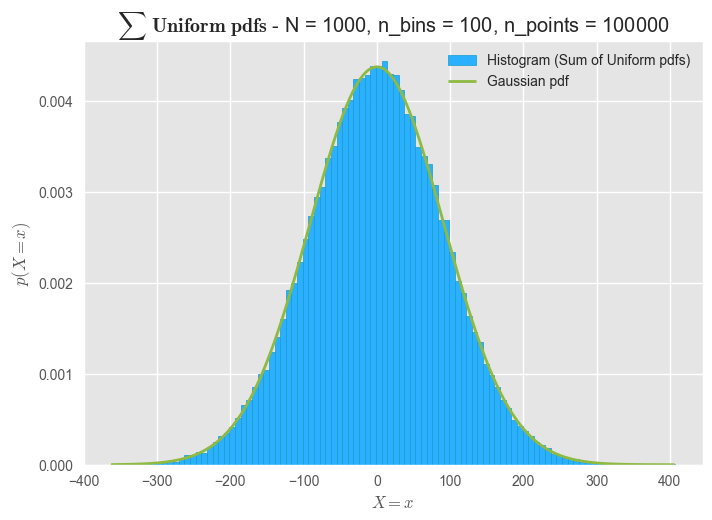
\includegraphics{vertopal_6d63c4420d4a47a4b64ec714b34abd06/014ec8a66ea44788e4837928af2d0d1e3b802589.png}

\hypertarget{gaussian-pdf}{%
\subsection{Gaussian pdf:}\label{gaussian-pdf}}

\begin{Shaded}
\begin{Highlighting}[]
\CommentTok{\# Definitions}
\NormalTok{N }\OperatorTok{=} \DecValTok{1\_000}\OperatorTok{;}\NormalTok{ n\_points }\OperatorTok{=} \DecValTok{100\_000}\OperatorTok{;}\NormalTok{ sum\_X\_vals }\OperatorTok{=}\NormalTok{ []}

\CommentTok{\# Initial Gaussian\textquotesingle{}s parameters}
\NormalTok{mu    }\OperatorTok{=} \DecValTok{0}
\NormalTok{sigma }\OperatorTok{=} \DecValTok{10}

\ControlFlowTok{for}\NormalTok{ n }\KeywordTok{in} \BuiltInTok{range}\NormalTok{(n\_points):}
\NormalTok{    X }\OperatorTok{=}\NormalTok{ np.random.normal(mu, sigma, N)}
\NormalTok{    sum\_X\_vals.append(}\BuiltInTok{sum}\NormalTok{(X))}
\end{Highlighting}
\end{Shaded}

\begin{Shaded}
\begin{Highlighting}[]
\CommentTok{\# Creating histogram}
\NormalTok{n\_bins }\OperatorTok{=} \DecValTok{100}
\NormalTok{hist, bins, \_ }\OperatorTok{=}\NormalTok{ plt.hist(sum\_X\_vals, density }\OperatorTok{=} \VariableTok{True}\NormalTok{, bins }\OperatorTok{=}\NormalTok{ n\_bins, label }\OperatorTok{=} \StringTok{\textquotesingle{}Histogram (Sum of Gaussian pdfs)\textquotesingle{}}\NormalTok{,}
\NormalTok{                         facecolor }\OperatorTok{=} \StringTok{\textquotesingle{}\#2ab0ff\textquotesingle{}}\NormalTok{, edgecolor}\OperatorTok{=}\StringTok{\textquotesingle{}\#169acf\textquotesingle{}}\NormalTok{, linewidth}\OperatorTok{=}\FloatTok{0.5}\NormalTok{) }\CommentTok{\# dimgray/maroon?}

\CommentTok{\# Analytic parameters (computed by hand)}
\NormalTok{mu\_X    }\OperatorTok{=} \DecValTok{0}
\NormalTok{sigma\_X }\OperatorTok{=}\NormalTok{ np.sqrt(N) }\OperatorTok{*} \DecValTok{10}

\NormalTok{x }\OperatorTok{=}\NormalTok{ np.linspace(bins.}\BuiltInTok{min}\NormalTok{(), bins.}\BuiltInTok{max}\NormalTok{(), }\DecValTok{1\_000}\NormalTok{)}
\NormalTok{plt.title(}\VerbatimStringTok{r\textquotesingle{}$\textbackslash{}sum$ $\textbackslash{}bf}\SpecialCharTok{\{Gaussian\}}\VerbatimStringTok{$ $\textbackslash{}bf}\SpecialCharTok{\{pdfs\}}\VerbatimStringTok{$ {-} \textquotesingle{}} \OperatorTok{+} \SpecialStringTok{f\textquotesingle{}N = }\SpecialCharTok{\{}\NormalTok{N}\SpecialCharTok{\}}\SpecialStringTok{, n\_bins = }\SpecialCharTok{\{}\NormalTok{n\_bins}\SpecialCharTok{\}}\SpecialStringTok{, n\_points = }\SpecialCharTok{\{}\NormalTok{n\_points}\SpecialCharTok{\}}\SpecialStringTok{\textquotesingle{}}\NormalTok{)}
\NormalTok{plt.plot(x, stats.norm.pdf(x, mu\_X, sigma\_X), label }\OperatorTok{=} \StringTok{\textquotesingle{}Gaussian pdf\textquotesingle{}}\NormalTok{, color }\OperatorTok{=} \StringTok{\textquotesingle{}C5\textquotesingle{}}\NormalTok{)}
\NormalTok{plt.xlabel(}\VerbatimStringTok{r\textquotesingle{}$X = x$\textquotesingle{}}\NormalTok{)}
\NormalTok{plt.ylabel(}\VerbatimStringTok{r\textquotesingle{}$p(X = x)$\textquotesingle{}}\NormalTok{)}
\NormalTok{plt.legend()}
\NormalTok{plt.show()}
\end{Highlighting}
\end{Shaded}

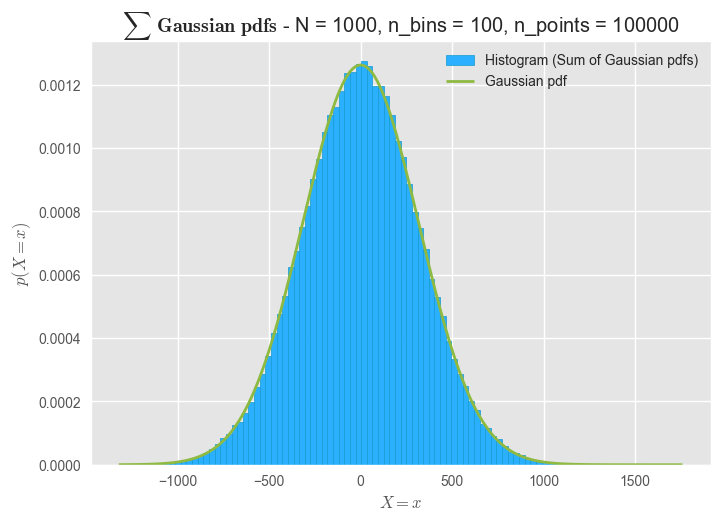
\includegraphics{vertopal_6d63c4420d4a47a4b64ec714b34abd06/3f50c84c72e85eb0d1af129acc1b3cd52b033a94.png}

\hypertarget{lorentzian-cauchy-pdf}{%
\subsection{Lorentzian (Cauchy) pdf:}\label{lorentzian-cauchy-pdf}}

\begin{itemize}
\tightlist
\item
  Here, the CLT is NOT valid!
\end{itemize}

\begin{Shaded}
\begin{Highlighting}[]
\CommentTok{\# Definitions}
\NormalTok{N }\OperatorTok{=} \DecValTok{1\_000}\OperatorTok{;}\NormalTok{ n\_points }\OperatorTok{=} \DecValTok{100\_000}\OperatorTok{;}\NormalTok{ sum\_X\_vals }\OperatorTok{=}\NormalTok{ []}

\CommentTok{\# Standard Cauchy distribution\textquotesingle{}s parameters. Not used in the code. Just here for reference/completeness.}
\NormalTok{x0    }\OperatorTok{=} \DecValTok{0}
\NormalTok{gamma }\OperatorTok{=} \DecValTok{1}

\ControlFlowTok{for}\NormalTok{ n }\KeywordTok{in} \BuiltInTok{range}\NormalTok{(n\_points):}
\NormalTok{    X }\OperatorTok{=}\NormalTok{ np.random.standard\_cauchy(N)}
\NormalTok{    X }\OperatorTok{=}\NormalTok{ X[(X}\OperatorTok{\textgreater{}{-}}\DecValTok{25}\NormalTok{) }\OperatorTok{\&}\NormalTok{ (X}\OperatorTok{\textless{}}\DecValTok{25}\NormalTok{)] }\CommentTok{\# Truncate distribution so it plots well}
\NormalTok{    sum\_X\_vals.append(}\BuiltInTok{sum}\NormalTok{(X))}
\end{Highlighting}
\end{Shaded}

\begin{Shaded}
\begin{Highlighting}[]
\CommentTok{\# Creating histogram}
\NormalTok{n\_bins }\OperatorTok{=} \DecValTok{100}
\NormalTok{hist, bins, \_ }\OperatorTok{=}\NormalTok{ plt.hist(sum\_X\_vals, density }\OperatorTok{=} \VariableTok{True}\NormalTok{, bins }\OperatorTok{=}\NormalTok{ n\_bins, label }\OperatorTok{=} \StringTok{\textquotesingle{}Histogram (Sum of Cauchy pdfs)\textquotesingle{}}\NormalTok{,}
\NormalTok{                         facecolor }\OperatorTok{=} \StringTok{\textquotesingle{}\#2ab0ff\textquotesingle{}}\NormalTok{, edgecolor}\OperatorTok{=}\StringTok{\textquotesingle{}\#169acf\textquotesingle{}}\NormalTok{, linewidth}\OperatorTok{=}\FloatTok{0.5}\NormalTok{) }\CommentTok{\# dimgray/maroon?}

\NormalTok{x }\OperatorTok{=}\NormalTok{ np.linspace(bins.}\BuiltInTok{min}\NormalTok{(), bins.}\BuiltInTok{max}\NormalTok{(), }\DecValTok{1\_000}\NormalTok{)}
\NormalTok{plt.title(}\VerbatimStringTok{r\textquotesingle{}$\textbackslash{}sum$ $\textbackslash{}bf}\SpecialCharTok{\{Cauchy\}}\VerbatimStringTok{$ $\textbackslash{}bf}\SpecialCharTok{\{pdfs\}}\VerbatimStringTok{$ {-} \textquotesingle{}} \OperatorTok{+} \SpecialStringTok{f\textquotesingle{}N = }\SpecialCharTok{\{}\NormalTok{N}\SpecialCharTok{\}}\SpecialStringTok{, n\_bins = }\SpecialCharTok{\{}\NormalTok{n\_bins}\SpecialCharTok{\}}\SpecialStringTok{, n\_points = }\SpecialCharTok{\{}\NormalTok{n\_points}\SpecialCharTok{\}}\SpecialStringTok{\textquotesingle{}}\NormalTok{)}
\NormalTok{plt.xlabel(}\VerbatimStringTok{r\textquotesingle{}$X = x$\textquotesingle{}}\NormalTok{)}
\NormalTok{plt.ylabel(}\VerbatimStringTok{r\textquotesingle{}$p(X = x)$\textquotesingle{}}\NormalTok{)}
\NormalTok{plt.legend()}
\NormalTok{plt.show()}
\end{Highlighting}
\end{Shaded}

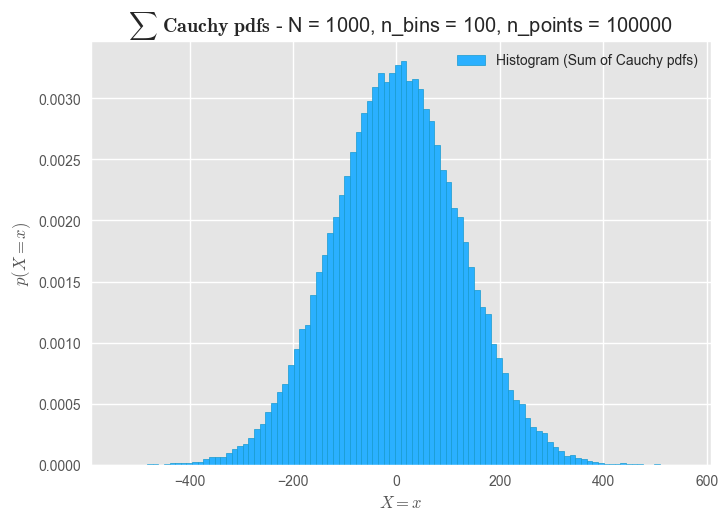
\includegraphics{vertopal_6d63c4420d4a47a4b64ec714b34abd06/18361d5674dc7f18513f81fcc770f096aa53916a.png}

\hypertarget{poisson-distribution}{%
\subsection{Poisson distribution:}\label{poisson-distribution}}

\begin{Shaded}
\begin{Highlighting}[]
\CommentTok{\# Definitions}
\NormalTok{N }\OperatorTok{=} \DecValTok{10\_000}\OperatorTok{;}\NormalTok{ n\_points }\OperatorTok{=} \DecValTok{100\_000}\OperatorTok{;}\NormalTok{ sum\_X\_vals }\OperatorTok{=}\NormalTok{ []}

\CommentTok{\# Poisson\textquotesingle{}s lambda parameter}
\NormalTok{lambda\_par }\OperatorTok{=} \DecValTok{1}

\ControlFlowTok{for}\NormalTok{ n }\KeywordTok{in} \BuiltInTok{range}\NormalTok{(n\_points):}
\NormalTok{    X }\OperatorTok{=}\NormalTok{ np.random.poisson(lambda\_par, N)}
\NormalTok{    sum\_X\_vals.append(}\BuiltInTok{sum}\NormalTok{(X))}
\end{Highlighting}
\end{Shaded}

\begin{Shaded}
\begin{Highlighting}[]
\CommentTok{\# Creating histogram}
\NormalTok{n\_bins }\OperatorTok{=} \DecValTok{100}
\NormalTok{hist, bins, \_ }\OperatorTok{=}\NormalTok{ plt.hist(sum\_X\_vals, density }\OperatorTok{=} \VariableTok{True}\NormalTok{, bins }\OperatorTok{=}\NormalTok{ n\_bins, label }\OperatorTok{=} \StringTok{\textquotesingle{}Histogram (Sum of Poisson distributions)\textquotesingle{}}\NormalTok{,}
\NormalTok{                         facecolor }\OperatorTok{=} \StringTok{\textquotesingle{}\#2ab0ff\textquotesingle{}}\NormalTok{, edgecolor}\OperatorTok{=}\StringTok{\textquotesingle{}\#169acf\textquotesingle{}}\NormalTok{, linewidth}\OperatorTok{=}\FloatTok{0.5}\NormalTok{) }\CommentTok{\# dimgray/maroon?}

\CommentTok{\# Analytic parameters (computed by hand)}
\NormalTok{mu    }\OperatorTok{=}\NormalTok{ N }\OperatorTok{*}\NormalTok{ lambda\_par}
\NormalTok{sigma }\OperatorTok{=}\NormalTok{ np.sqrt(N }\OperatorTok{*}\NormalTok{ lambda\_par)}

\NormalTok{x }\OperatorTok{=}\NormalTok{ np.linspace(bins.}\BuiltInTok{min}\NormalTok{(), bins.}\BuiltInTok{max}\NormalTok{(), }\DecValTok{1\_000}\NormalTok{)}
\NormalTok{plt.title(}\VerbatimStringTok{r\textquotesingle{}$\textbackslash{}sum$ $\textbackslash{}bf}\SpecialCharTok{\{Poisson\}}\VerbatimStringTok{$ $\textbackslash{}bf}\SpecialCharTok{\{distributions\}}\VerbatimStringTok{$ {-} \textquotesingle{}} \OperatorTok{+} \SpecialStringTok{f\textquotesingle{}N = }\SpecialCharTok{\{}\NormalTok{N}\SpecialCharTok{\}}\SpecialStringTok{, n\_bins = }\SpecialCharTok{\{}\NormalTok{n\_bins}\SpecialCharTok{\}}\SpecialStringTok{, n\_points = }\SpecialCharTok{\{}\NormalTok{n\_points}\SpecialCharTok{\}}\SpecialStringTok{\textquotesingle{}}\NormalTok{)}
\NormalTok{plt.plot(x, stats.norm.pdf(x, mu, sigma), label }\OperatorTok{=} \StringTok{\textquotesingle{}Gaussian pdf\textquotesingle{}}\NormalTok{, color }\OperatorTok{=} \StringTok{\textquotesingle{}C5\textquotesingle{}}\NormalTok{)}
\NormalTok{plt.xlabel(}\VerbatimStringTok{r\textquotesingle{}$X = x$\textquotesingle{}}\NormalTok{)}
\NormalTok{plt.ylabel(}\VerbatimStringTok{r\textquotesingle{}$p(X = x)$\textquotesingle{}}\NormalTok{)}
\NormalTok{plt.legend()}
\NormalTok{plt.show()}
\end{Highlighting}
\end{Shaded}

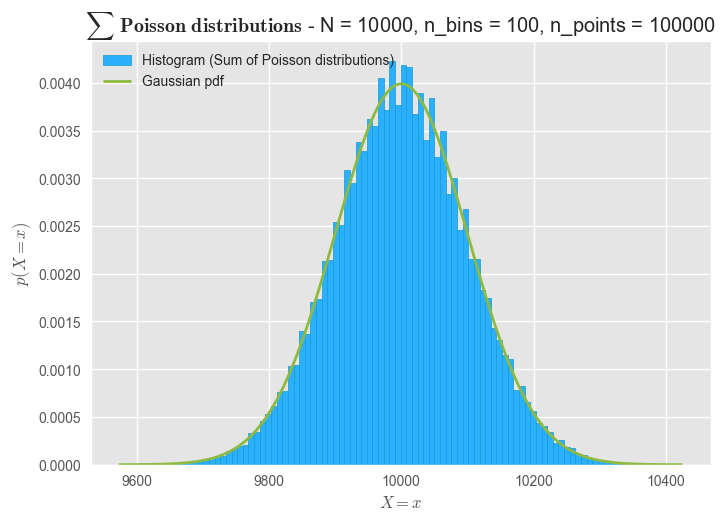
\includegraphics{vertopal_6d63c4420d4a47a4b64ec714b34abd06/7e3e3c7f87cd19bb9cc16a1598cf3329ece30ce8.png}

As can be seen from the plots, the Central Limit Theorem (CLT) is
verified, except for the Cauchy distribution. In fact, this
distribution\textquotesingle s mean and variance are not defined. As
such, we cannot expect the CLT to hold.

\end{document}
